\documentclass[border=12pt]{standalone}
\usepackage{amsmath}
\usepackage{tikz}
\usetikzlibrary{arrows.meta,positioning}
\begin{document}
\begin{tabular}{c@{\hskip 1.4cm}c@{\hskip 1.4cm}c}
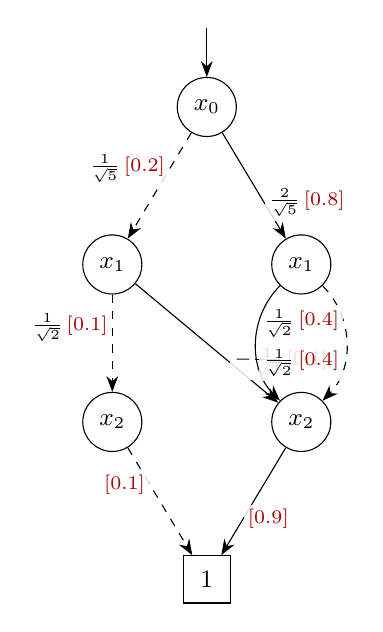
\begin{tikzpicture}[
    every node/.style={font=\small},
    nd/.style={circle, draw, minimum size=7.5mm, inner sep=0pt},
    tm/.style={rectangle, draw, minimum size=6mm, inner sep=2pt},
    e/.style={-{Stealth[length=2mm]}},
    lbl/.style={font=\scriptsize, inner sep=1.5pt, fill=white,
                fill opacity=0.85, text opacity=1},
    idl/.style={font=\tiny, inner sep=1pt, gray},
  ]
  \node[nd] (n5) at (0.00, 0.00) {$x_{0}$};
  \node[nd] (n3) at (-1.20, -2.00) {$x_{1}$};
  \node[nd] (n4) at (1.20, -2.00) {$x_{1}$};
  \node[nd] (n1) at (-1.20, -4.00) {$x_{2}$};
  \node[nd] (n2) at (1.20, -4.00) {$x_{2}$};
  \node[tm] (term) at (0, -6.00) {$1$};
  \coordinate (in) at (0.00, 1.00);
  \draw[e] (in) -- (n5);
  \draw[e, dashed] (n1) -- node[lbl, left, pos=0.34] {{\color{red!65!black}[0.1]}} (term);
  \draw[e, solid] (n2) -- node[lbl, right, pos=0.66] {{\color{red!65!black}[0.9]}} (term);
  \draw[e, dashed] (n3) -- node[lbl, left, pos=0.34] {$\tfrac{1}{\sqrt{2}}$\,{\color{red!65!black}[0.1]}} (n1);
  \draw[e, solid] (n3) -- node[lbl, right, pos=0.66] {$-\tfrac{1}{\sqrt{2}}$\,{\color{red!65!black}[0.1]}} (n2);
  \draw[e, dashed] (n4) to[bend left=45] node[lbl, left, pos=0.34] {$\tfrac{1}{\sqrt{2}}$\,{\color{red!65!black}[0.4]}} (n2);
  \draw[e, solid] (n4) to[bend right=45] node[lbl, right, pos=0.66] {$\tfrac{1}{\sqrt{2}}$\,{\color{red!65!black}[0.4]}} (n2);
  \draw[e, dashed] (n5) -- node[lbl, left, pos=0.34] {$\tfrac{1}{\sqrt{5}}$\,{\color{red!65!black}[0.2]}} (n3);
  \draw[e, solid] (n5) -- node[lbl, right, pos=0.66] {$\tfrac{2}{\sqrt{5}}$\,{\color{red!65!black}[0.8]}} (n4);
\end{tikzpicture}
&
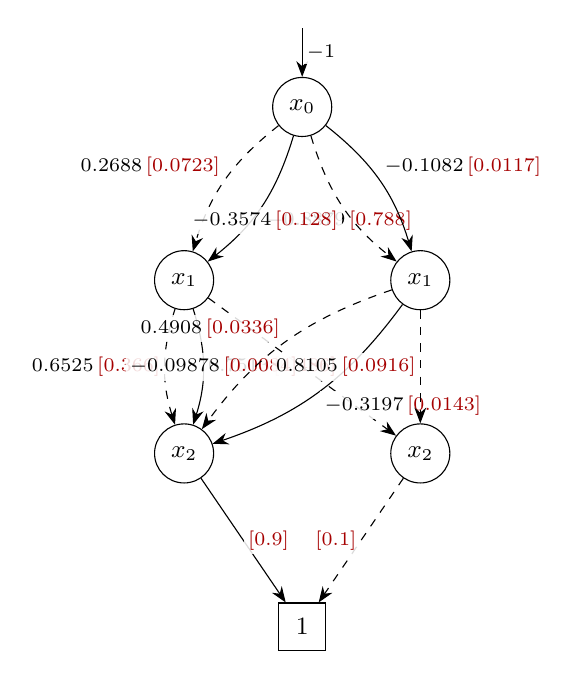
\begin{tikzpicture}[
    every node/.style={font=\small},
    nd/.style={circle, draw, minimum size=7.5mm, inner sep=0pt},
    tm/.style={rectangle, draw, minimum size=6mm, inner sep=2pt},
    e/.style={-{Stealth[length=2mm]}},
    lbl/.style={font=\scriptsize, inner sep=1.5pt, fill=white,
                fill opacity=0.85, text opacity=1},
    idl/.style={font=\tiny, inner sep=1pt, gray},
  ]
  \node[nd] (n5) at (0.00, 0.00) {$x_{0}$};
  \node[nd] (n3) at (-1.50, -2.20) {$x_{1}$};
  \node[nd] (n4) at (1.50, -2.20) {$x_{1}$};
  \node[nd] (n1) at (-1.50, -4.40) {$x_{2}$};
  \node[nd] (n2) at (1.50, -4.40) {$x_{2}$};
  \node[tm] (term) at (0, -6.60) {$1$};
  \coordinate (in) at (0.00, 1.00);
  \draw[e, solid] (in) -- node[lbl, right] {$-1$} (n5);
  \draw[e, dashed] (n5) to[bend right=17.5] node[lbl, auto, swap, pos=0.5] {$0.2688$\,{\color{red!65!black}[0.0723]}} (n3);
  \draw[e, solid] (n5) to[bend left=17.5] node[lbl, auto, pos=0.5] {$-0.8879$\,{\color{red!65!black}[0.788]}} (n3);
  \draw[e, dashed] (n5) to[bend right=17.5] node[lbl, auto, swap, pos=0.5] {$-0.3574$\,{\color{red!65!black}[0.128]}} (n4);
  \draw[e, solid] (n5) to[bend left=17.5] node[lbl, auto, pos=0.5] {$-0.1082$\,{\color{red!65!black}[0.0117]}} (n4);
  \draw[e, dashed] (n3) to[bend right=17.5] node[lbl, auto, swap, pos=0.5] {$0.6525$\,{\color{red!65!black}[0.366]}} (n1);
  \draw[e, solid] (n3) to[bend left=17.5] node[lbl, auto, pos=0.5] {$0.7513$\,{\color{red!65!black}[0.486]}} (n1);
  \draw[e, dashed] (n3) -- node[lbl, left, pos=0.5] {$-0.09878$\,{\color{red!65!black}[0.0084]}} (n2);
  \draw[e, dashed] (n4) to[bend right=17.5] node[lbl, auto, swap, pos=0.5] {$0.4908$\,{\color{red!65!black}[0.0336]}} (n1);
  \draw[e, solid] (n4) to[bend left=17.5] node[lbl, auto, pos=0.5] {$-0.3197$\,{\color{red!65!black}[0.0143]}} (n1);
  \draw[e, dashed] (n4) -- node[lbl, left, pos=0.5] {$0.8105$\,{\color{red!65!black}[0.0916]}} (n2);
  \draw[e, solid] (n1) -- node[lbl, right, pos=0.5] {{\color{red!65!black}[0.9]}} (term);
  \draw[e, dashed] (n2) -- node[lbl, left, pos=0.5] {{\color{red!65!black}[0.1]}} (term);
\end{tikzpicture}
&

\\[4pt] exact: 5 nodes & exact nd-EVDD from TT (non-deterministic): 5 nodes, 12 edges & 
\\[10pt]
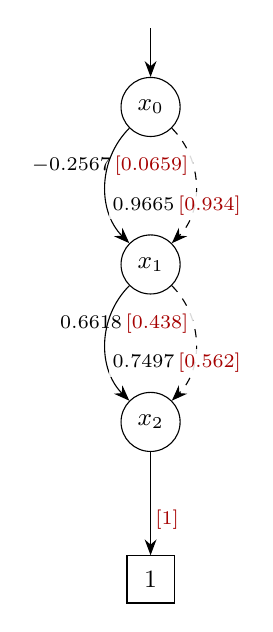
\begin{tikzpicture}[
    every node/.style={font=\small},
    nd/.style={circle, draw, minimum size=7.5mm, inner sep=0pt},
    tm/.style={rectangle, draw, minimum size=6mm, inner sep=2pt},
    e/.style={-{Stealth[length=2mm]}},
    lbl/.style={font=\scriptsize, inner sep=1.5pt, fill=white,
                fill opacity=0.85, text opacity=1},
    idl/.style={font=\tiny, inner sep=1pt, gray},
  ]
  \node[nd] (n3) at (0.00, 0.00) {$x_{0}$};
  \node[nd] (n2) at (0.00, -2.00) {$x_{1}$};
  \node[nd] (n1) at (0.00, -4.00) {$x_{2}$};
  \node[tm] (term) at (0, -6.00) {$1$};
  \coordinate (in) at (0.00, 1.00);
  \draw[e] (in) -- (n3);
  \draw[e, solid] (n1) -- node[lbl, right, pos=0.66] {{\color{red!65!black}[1]}} (term);
  \draw[e, dashed] (n2) to[bend left=45] node[lbl, left, pos=0.34] {$0.6618$\,{\color{red!65!black}[0.438]}} (n1);
  \draw[e, solid] (n2) to[bend right=45] node[lbl, right, pos=0.66] {$0.7497$\,{\color{red!65!black}[0.562]}} (n1);
  \draw[e, dashed] (n3) to[bend left=45] node[lbl, left, pos=0.34] {$-0.2567$\,{\color{red!65!black}[0.0659]}} (n2);
  \draw[e, solid] (n3) to[bend right=45] node[lbl, right, pos=0.66] {$0.9665$\,{\color{red!65!black}[0.934]}} (n2);
\end{tikzpicture}
&
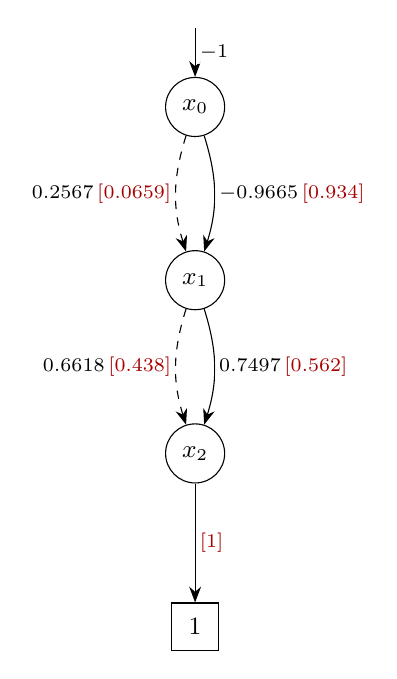
\begin{tikzpicture}[
    every node/.style={font=\small},
    nd/.style={circle, draw, minimum size=7.5mm, inner sep=0pt},
    tm/.style={rectangle, draw, minimum size=6mm, inner sep=2pt},
    e/.style={-{Stealth[length=2mm]}},
    lbl/.style={font=\scriptsize, inner sep=1.5pt, fill=white,
                fill opacity=0.85, text opacity=1},
    idl/.style={font=\tiny, inner sep=1pt, gray},
  ]
  \node[nd] (n3) at (0.00, 0.00) {$x_{0}$};
  \node[nd] (n2) at (0.00, -2.20) {$x_{1}$};
  \node[nd] (n1) at (0.00, -4.40) {$x_{2}$};
  \node[tm] (term) at (0, -6.60) {$1$};
  \coordinate (in) at (0.00, 1.00);
  \draw[e, solid] (in) -- node[lbl, right] {$-1$} (n3);
  \draw[e, dashed] (n3) to[bend right=17.5] node[lbl, auto, swap, pos=0.5] {$0.2567$\,{\color{red!65!black}[0.0659]}} (n2);
  \draw[e, solid] (n3) to[bend left=17.5] node[lbl, auto, pos=0.5] {$-0.9665$\,{\color{red!65!black}[0.934]}} (n2);
  \draw[e, dashed] (n2) to[bend right=17.5] node[lbl, auto, swap, pos=0.5] {$0.6618$\,{\color{red!65!black}[0.438]}} (n1);
  \draw[e, solid] (n2) to[bend left=17.5] node[lbl, auto, pos=0.5] {$0.7497$\,{\color{red!65!black}[0.562]}} (n1);
  \draw[e, solid] (n1) -- node[lbl, right, pos=0.5] {{\color{red!65!black}[1]}} (term);
\end{tikzpicture}
&
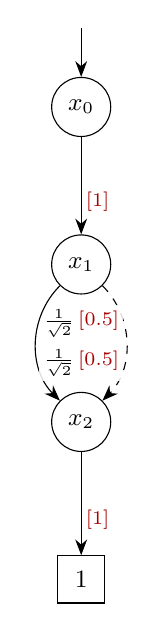
\begin{tikzpicture}[
    every node/.style={font=\small},
    nd/.style={circle, draw, minimum size=7.5mm, inner sep=0pt},
    tm/.style={rectangle, draw, minimum size=6mm, inner sep=2pt},
    e/.style={-{Stealth[length=2mm]}},
    lbl/.style={font=\scriptsize, inner sep=1.5pt, fill=white,
                fill opacity=0.85, text opacity=1},
    idl/.style={font=\tiny, inner sep=1pt, gray},
  ]
  \node[nd] (n8) at (0.00, 0.00) {$x_{0}$};
  \node[nd] (n4) at (0.00, -2.00) {$x_{1}$};
  \node[nd] (n2) at (0.00, -4.00) {$x_{2}$};
  \node[tm] (term) at (0, -6.00) {$1$};
  \coordinate (in) at (0.00, 1.00);
  \draw[e] (in) -- (n8);
  \draw[e, solid] (n2) -- node[lbl, right, pos=0.66] {{\color{red!65!black}[1]}} (term);
  \draw[e, dashed] (n4) to[bend left=45] node[lbl, left, pos=0.34] {$\tfrac{1}{\sqrt{2}}$\,{\color{red!65!black}[0.5]}} (n2);
  \draw[e, solid] (n4) to[bend right=45] node[lbl, right, pos=0.66] {$\tfrac{1}{\sqrt{2}}$\,{\color{red!65!black}[0.5]}} (n2);
  \draw[e, solid] (n8) -- node[lbl, right, pos=0.66] {{\color{red!65!black}[1]}} (n4);
\end{tikzpicture}
\\[4pt] $\chi=1$, TT $\to$ det: 3 nodes, $F=0.853$ & nd-EVDD from TT: 3 nodes, 5 edges & Hillmich $f=0.800$: 3 nodes, $F=0.800$
\end{tabular}
\end{document}